%results


The cross sections of $^{3}$He, $^{4}$He and $^{12}$C at scattering angle of $25^{\circ}$ are shown in Fig.~\ref{xs}.
{\bf say more about the figure when we have the final one}

                \begin{figure}[!ht]
		\begin{center}
		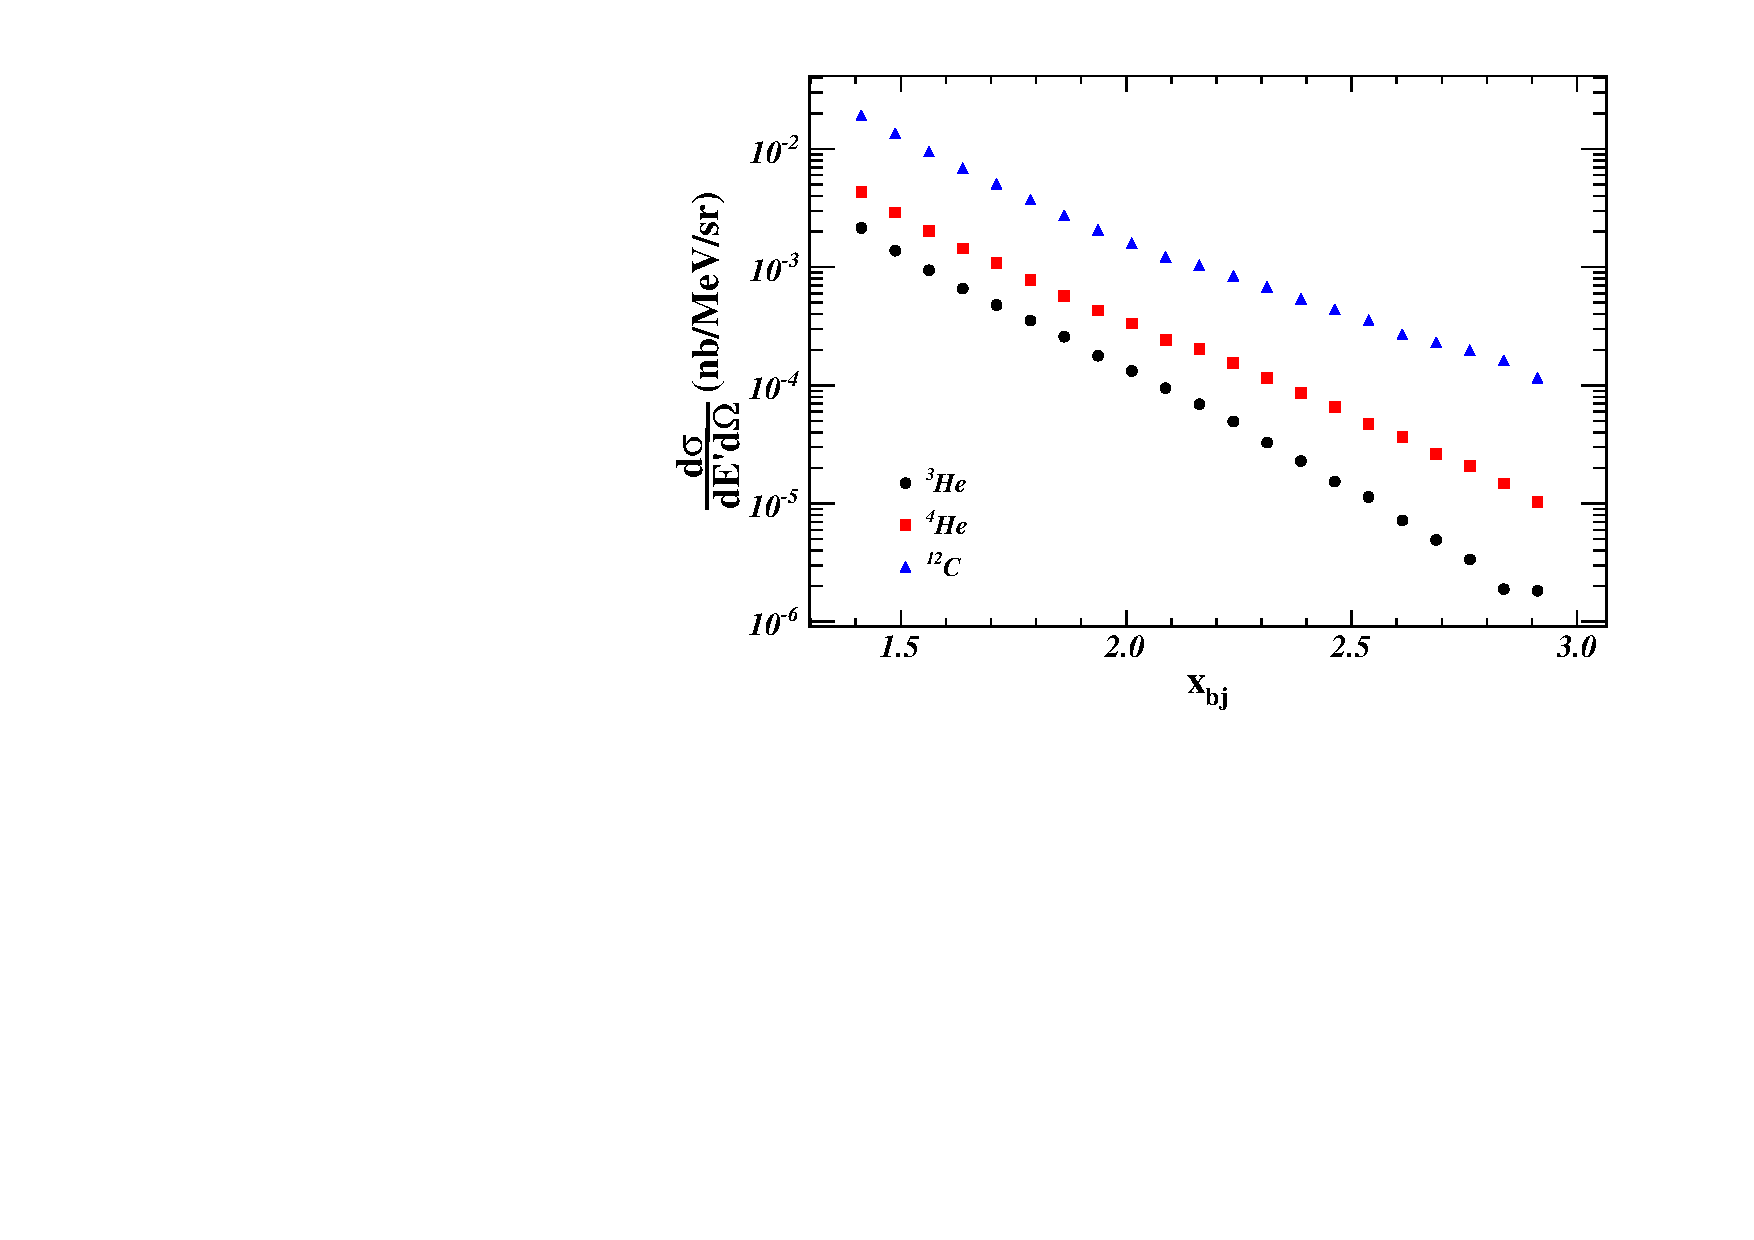
\includegraphics[width=9.5cm]{./figures/XS_Comp_25_May27.pdf}
		\end{center}
		\vspace*{-5mm}
		\caption{Cross sections of $^{3}$He, $^{4}$He and $^{12}$C at $25^{\circ}$. Statistical errors and
                  systematic errors from instruments are included.}
		\label{xs}
		\end{figure}


                \begin{figure}[!ht]
		\begin{center}
		  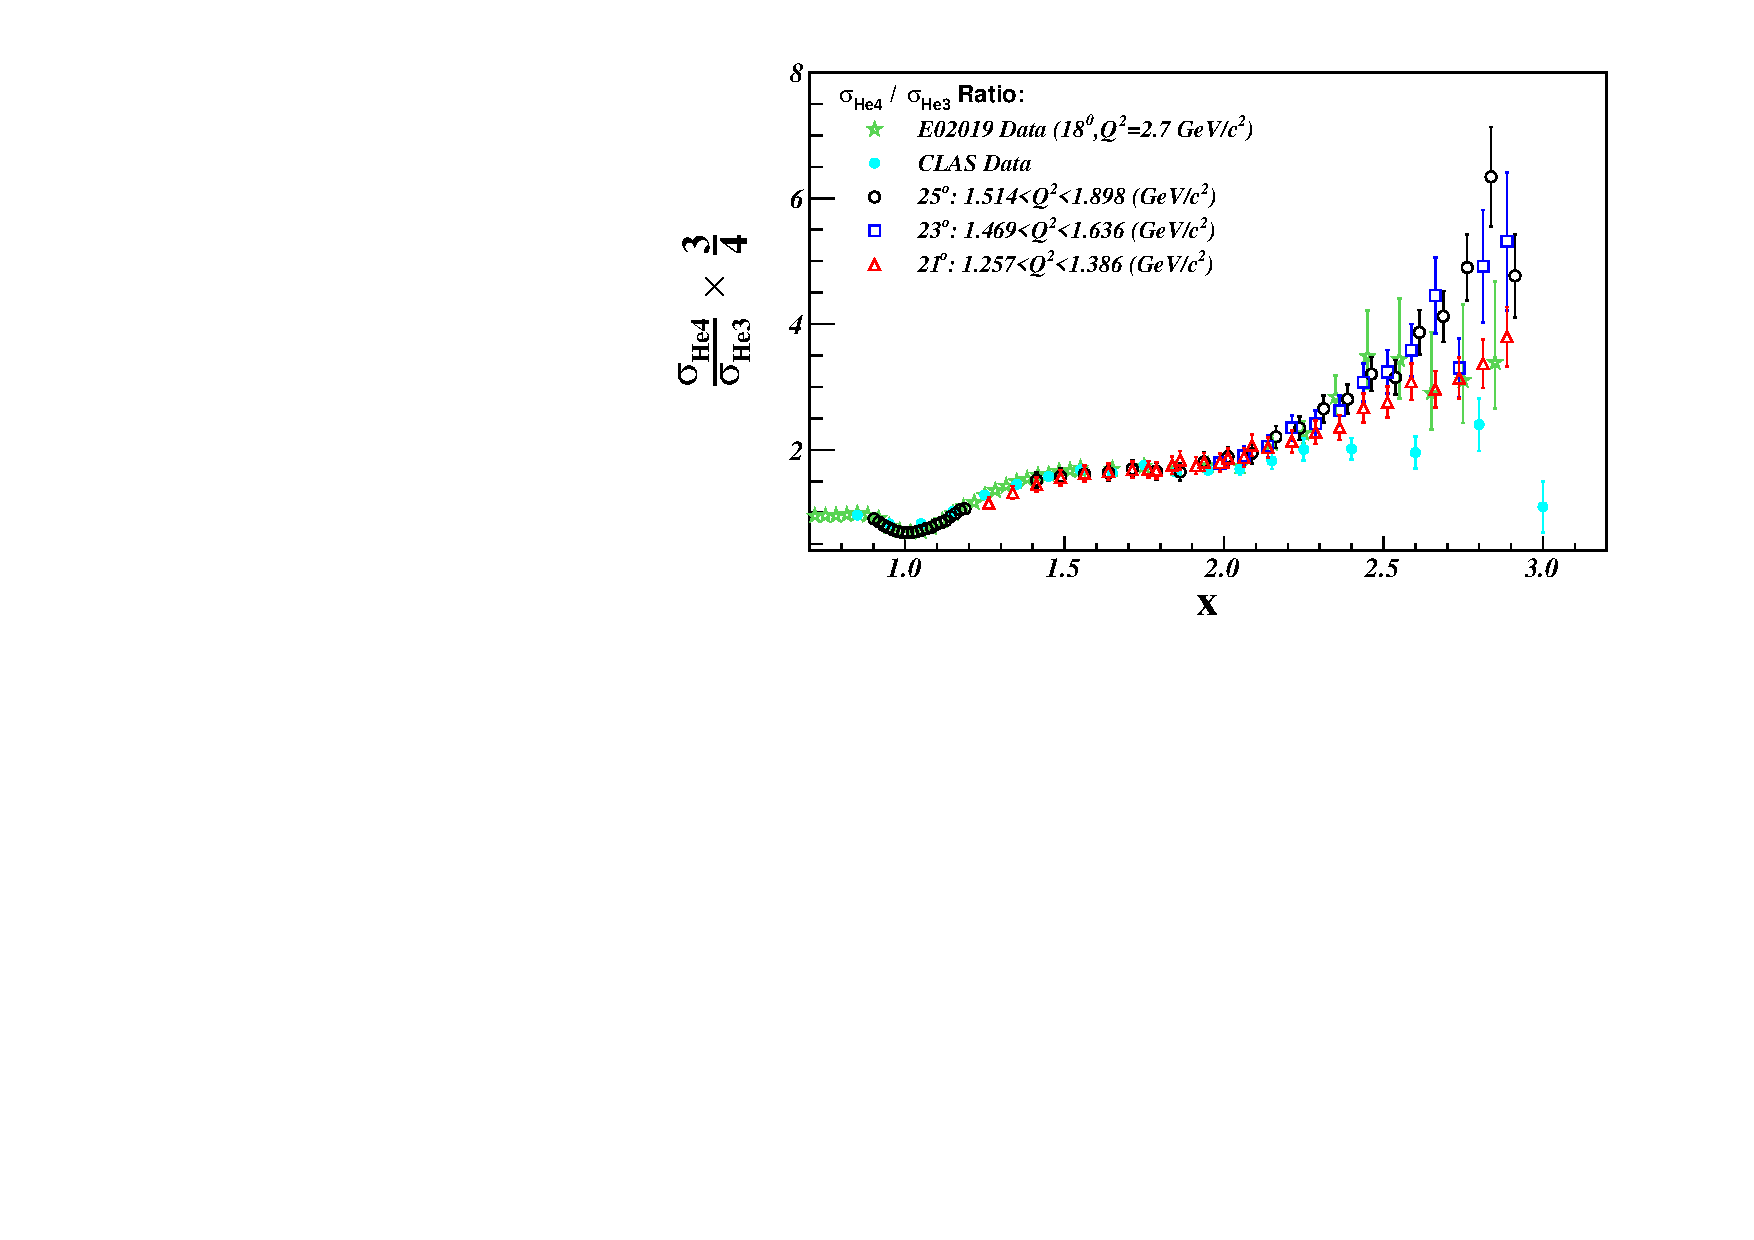
\includegraphics[width=9.5cm]{./figures/He4_He3_XS_Ratio_June30_L.pdf}
                  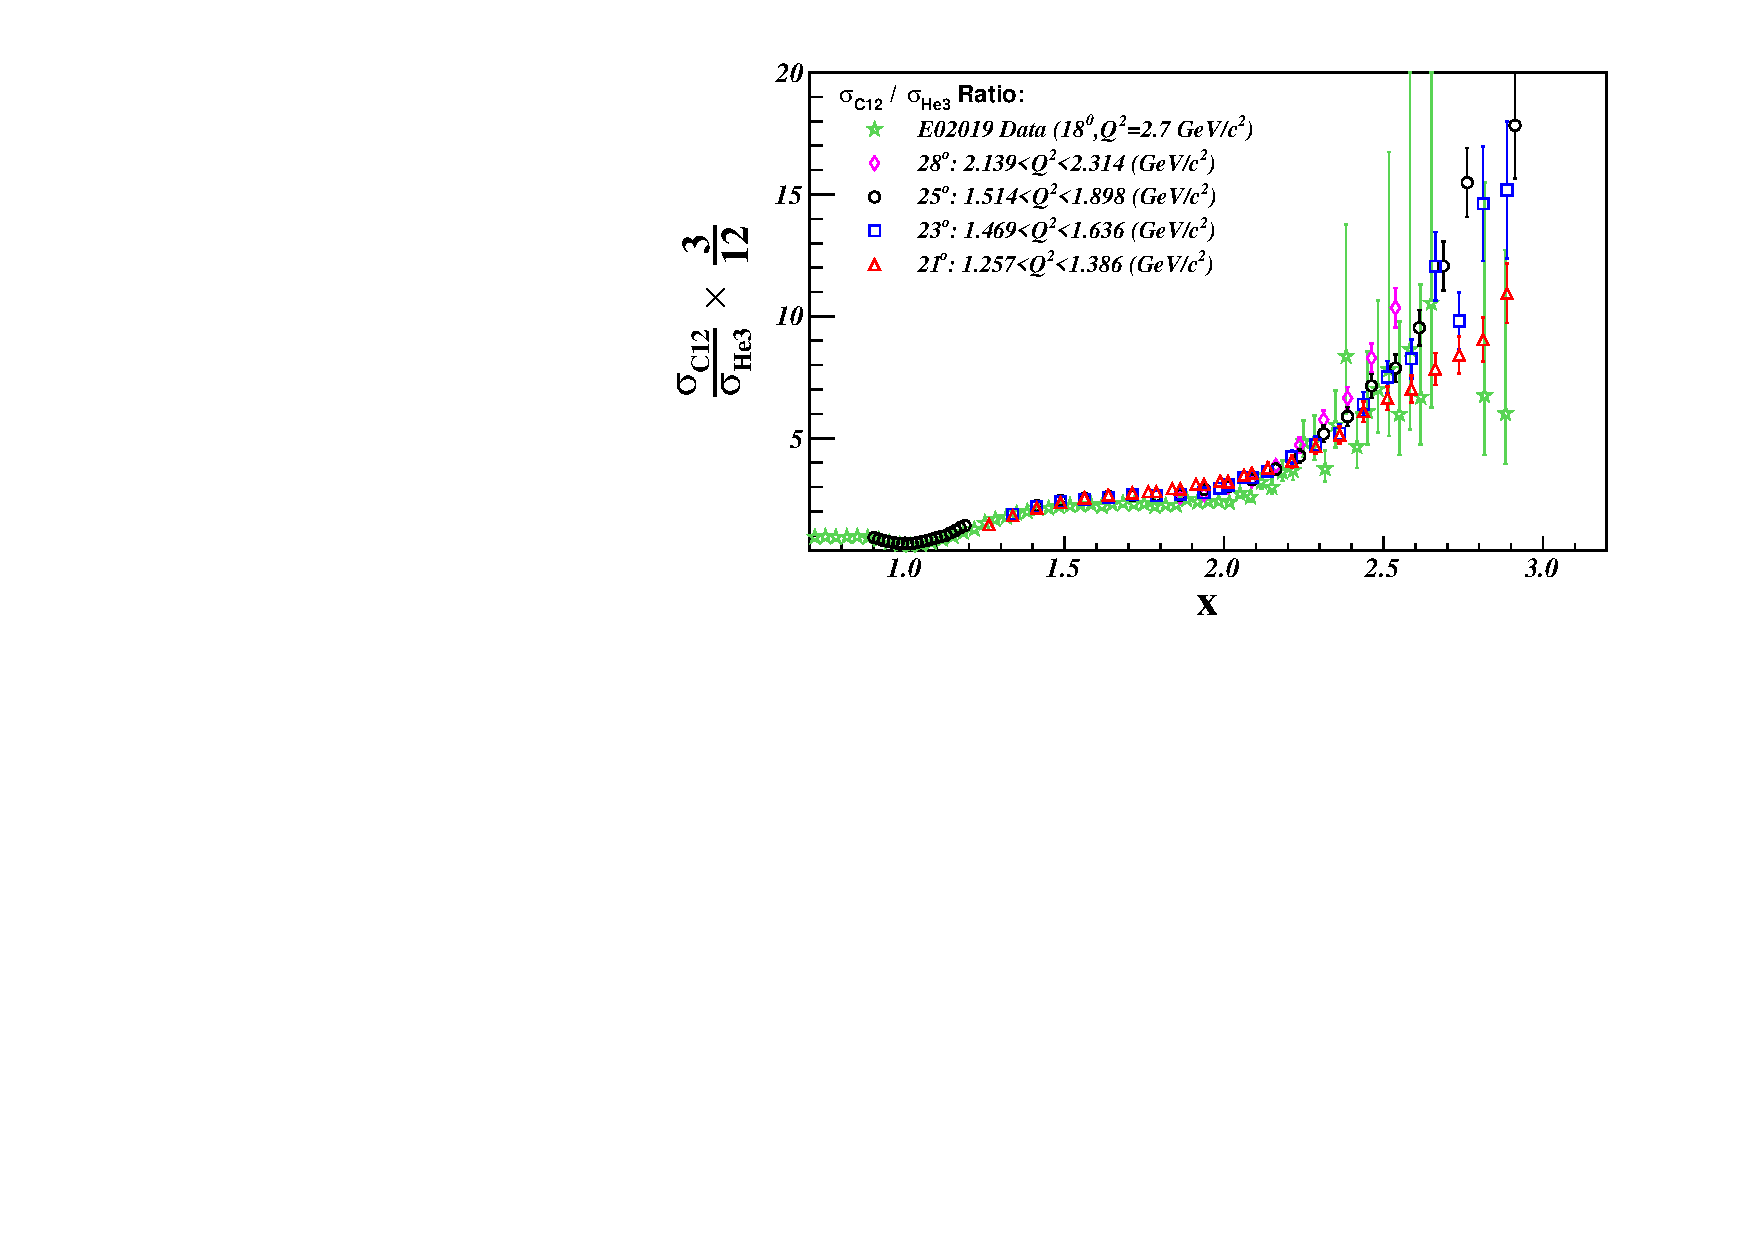
\includegraphics[width=9.5cm]{./figures/C12_He3_XS_Ratio_June30_L.pdf}
                  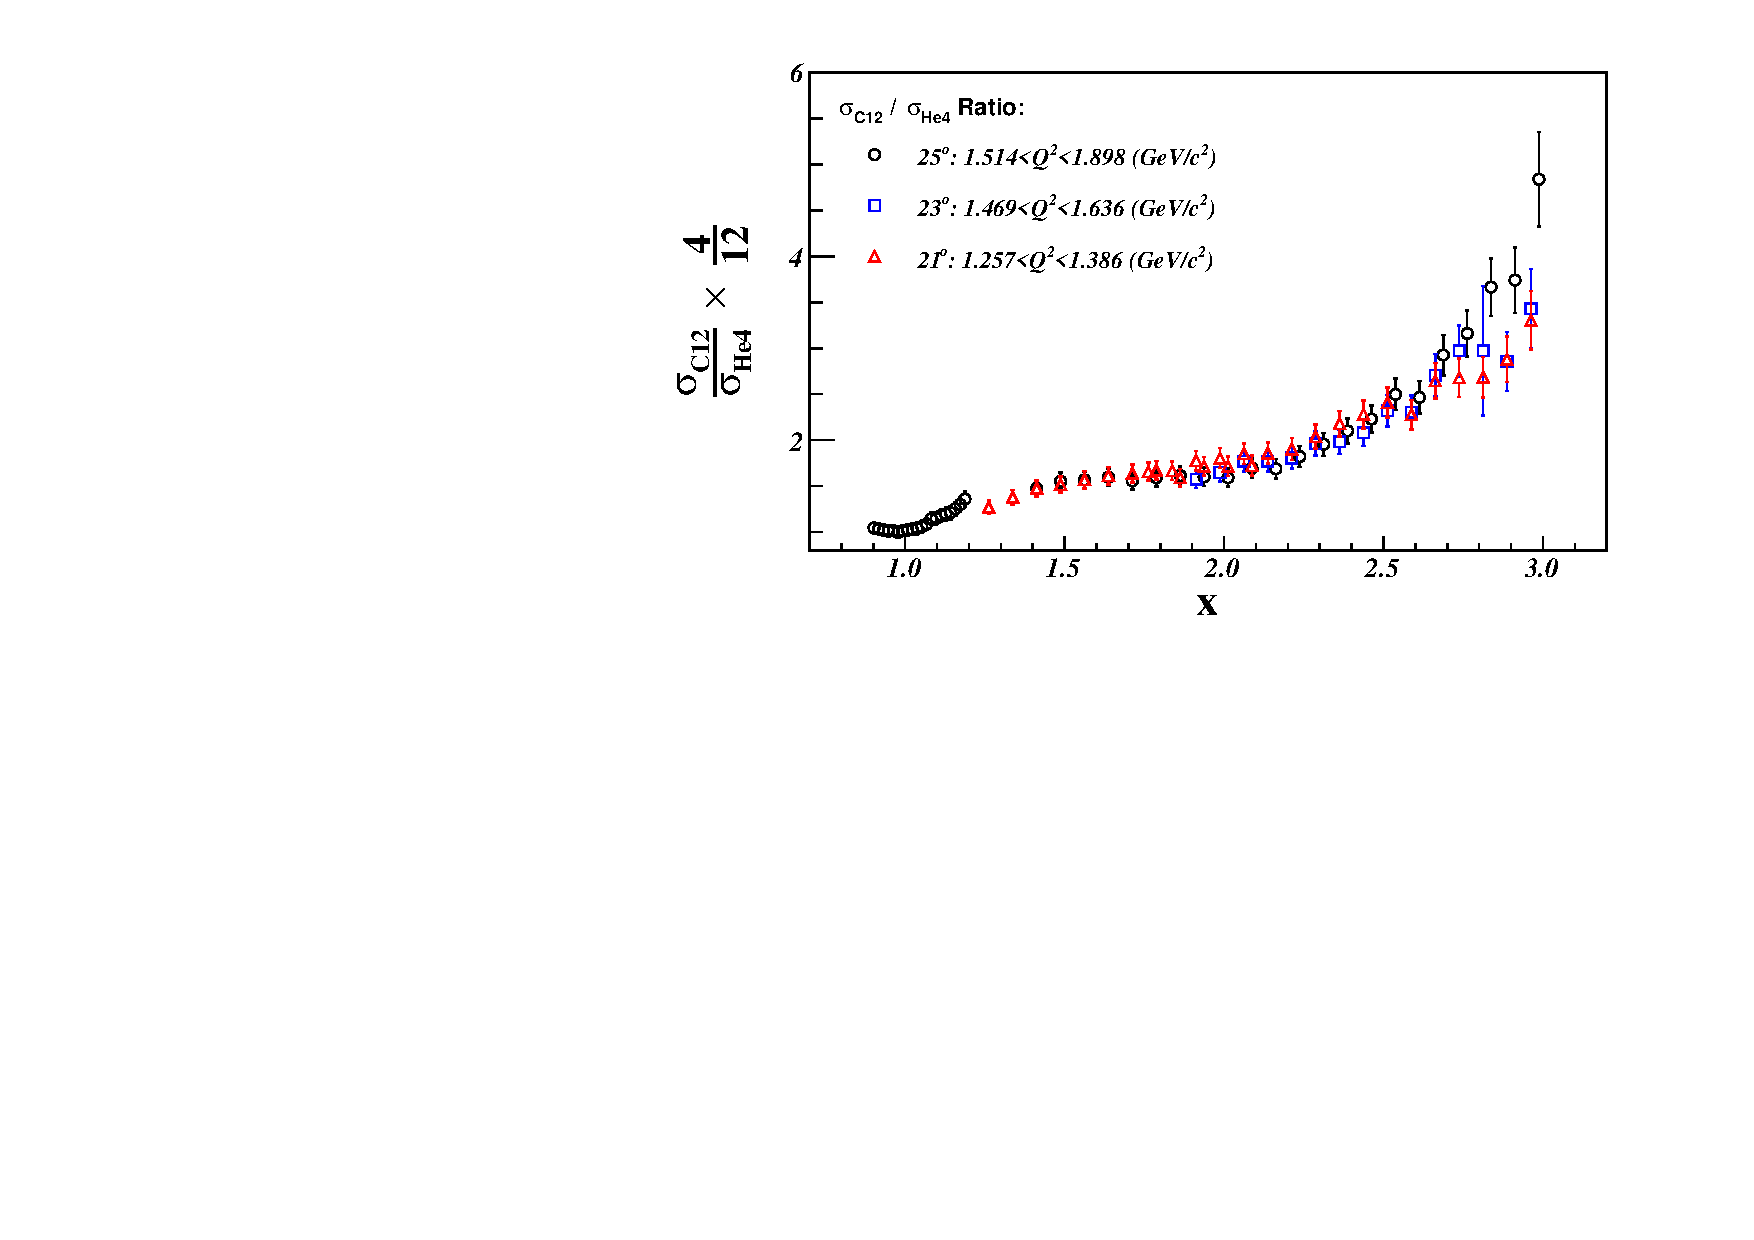
\includegraphics[width=9.5cm]{./figures/C12_He4_XS_Ratio_June30_L.pdf}
		\end{center}
		\vspace*{-5mm}
		\caption{{\bf Top: } Cross section ratio of $^{4}$He to $^{3}$He with this experiment at three $Q^{2}$
                  settings and also the results from JLab E02-019 and CLAS. {\bf Middle: } Cross section ratio of
                  $^{12}$C to $^{3}$He with this experiment at four $Q^{2}$ settings and also the results from JLab
                  E02-019. {\bf Bottom:} Cross section ratio of $^{12}$C to $^{4}$He with this experiment at three
                  $Q^{2}$ settings.
                  In all plots, Statistical errors and systematic errors are included.}
		\label{ratios}
		\end{figure}

Fig.~\ref{ratios} presents the cross section ratios of $\mathrm{^{4}He}$ to $\mathrm{^{3}He}$, $\mathrm{^{12}C}$ to $\mathrm{^{3}He}$
and $\mathrm{^{12}C}$ to $\mathrm{^{4}He}$ as a function of $x$. In the 2N-SRC region, our data are in great agreement with the data
from JLab E02-019 and CLAS, revealing a plateau between $x \approx 1.5$ and $x = 2$. However, at $x>2$, no hint of a 3N-SRC plateau
is visible. Instead our data continue rising up quickly when $x$ approaches 3, showing the same trend the E02-019 data. While E02-019
ran at higher $\mathrm{Q^{2}}$, our data and the CLAS data were taken in the similar $\mathrm{Q^{2}}$-range but yield different
approaches. A recent publication suggested that the 3N-SRC plateau showed in the CLAS data could be a result of inappropriate
binning and bin-centering correction~\cite{Higinbotham:2014xna}.
